\documentclass[a4paper, 14pt]{extarticle}

% Поля
%--------------------------------------
\usepackage{geometry}
\geometry{a4paper,tmargin=2cm,bmargin=2cm,lmargin=3cm,rmargin=1cm}
%--------------------------------------


%Russian-specific packages
%--------------------------------------
\usepackage[T2A]{fontenc}
\usepackage[utf8]{inputenc} 
\usepackage[english, main=russian]{babel}
%--------------------------------------

\usepackage{textcomp}

% Красная строка
%--------------------------------------
\usepackage{indentfirst}               
%--------------------------------------             

\newcommand{\T}{\mathcal{T}}

%Graphics
%--------------------------------------
\usepackage{graphicx}
\graphicspath{ {./images/} }
\usepackage{wrapfig}
%--------------------------------------

% Полуторный интервал
%--------------------------------------
\linespread{1.3}                    
%--------------------------------------

%Выравнивание и переносы
%--------------------------------------
% Избавляемся от переполнений
\sloppy
% Запрещаем разрыв страницы после первой строки абзаца
\clubpenalty=10000
% Запрещаем разрыв страницы после последней строки абзаца
\widowpenalty=10000
%--------------------------------------

%Списки
\usepackage{enumitem}

%Подписи
\usepackage{caption} 

%Гиперссылки
\usepackage{hyperref}

\hypersetup {
	unicode=true
}

%Рисунки
%--------------------------------------
\DeclareCaptionLabelSeparator*{emdash}{~--- }
\captionsetup[figure]{labelsep=emdash,font=onehalfspacing,position=bottom}
%--------------------------------------

\usepackage{tempora}


%Листинги
%--------------------------------------
\usepackage{listings}
\lstset{
  basicstyle=\ttfamily\footnotesize, 
  %basicstyle=\footnotesize\AnkaCoder,        % the size of the fonts that are used for the code
  breakatwhitespace=false,         % sets if automatic breaks shoulbd only happen at whitespace
  breaklines=true,                 % sets automatic line breaking
  captionpos=t,                    % sets the caption-position to bottom
  inputencoding=utf8,
  frame=single,                    % adds a frame around the code
  keepspaces=true,                 % keeps spaces in text, useful for keeping indentation of code (possibly needs columns=flexible)
  keywordstyle=\bf,       % keyword style
  numbers=left,                    % where to put the line-numbers; possible values are (none, left, right)
  numbersep=5pt,                   % how far the line-numbers are from the code
  xleftmargin=25pt,
  xrightmargin=25pt,
  showspaces=false,                % show spaces everywhere adding particular underscores; it overrides 'showstringspaces'
  showstringspaces=false,          % underline spaces within strings only
  showtabs=false,                  % show tabs within strings adding particular underscores
  stepnumber=1,                    % the step between two line-numbers. If it's 1, each line will be numbered
  tabsize=2,                       % sets default tabsize to 8 spaces
  title=\lstname                   % show the filename of files included with \lstinputlisting; also try caption instead of title
}

%--------------------------------------

%%% Математические пакеты %%%
%--------------------------------------
\usepackage{amsthm,amsfonts,amsmath,amssymb,amscd}  % Математические дополнения от AMS
\usepackage{mathtools}                              % Добавляет окружение multlined
\usepackage[perpage]{footmisc}
%--------------------------------------

%--------------------------------------
%			НАЧАЛО ДОКУМЕНТА
%--------------------------------------

\begin{document}

%--------------------------------------
%			ТИТУЛЬНЫЙ ЛИСТ
%--------------------------------------
% \begin{titlepage}
% \thispagestyle{empty}
% \newpage


% %Шапка титульного листа
% %--------------------------------------
% \vspace*{-60pt}
% \hspace{-65pt}
% \begin{minipage}{0.3\textwidth}
% \hspace*{-20pt}\centering
% 
\includegraphics[width=\textwidth]{emblem}
% \end{minipage}
% \begin{minipage}{0.67\textwidth}\small \textbf{
% \vspace*{-0.7ex}
% \hspace*{-6pt}\centerline{Министерство науки и высшего образования Российской Федерации}
% \vspace*{-0.7ex}
% \centerline{Федеральное государственное бюджетное образовательное учреждение }
% \vspace*{-0.7ex}
% \centerline{высшего образования}
% \vspace*{-0.7ex}
% \centerline{<<Московский государственный технический университет}
% \vspace*{-0.7ex}
% \centerline{имени Н.Э. Баумана}
% \vspace*{-0.7ex}
% \centerline{(национальный исследовательский университет)>>}
% \vspace*{-0.7ex}
% \centerline{(МГТУ им. Н.Э. Баумана)}}
% \end{minipage}
% %--------------------------------------

% %Полосы
% %--------------------------------------
% \vspace{-25pt}
% \hspace{-35pt}\rule{\textwidth}{2.3pt}

% \vspace*{-20.3pt}
% \hspace{-35pt}\rule{\textwidth}{0.4pt}
% %--------------------------------------

% \vspace{1.5ex}
% \hspace{-35pt} \noindent \small ФАКУЛЬТЕТ\hspace{80pt} <<Информатика и системы управления>>

% \vspace*{-16pt}
% \hspace{47pt}\rule{0.83\textwidth}{0.4pt}

% \vspace{0.5ex}
% \hspace{-35pt} \noindent \small КАФЕДРА\hspace{50pt} <<Теоретическая информатика и компьютерные технологии>>

% \vspace*{-16pt}
% \hspace{30pt}\rule{0.866\textwidth}{0.4pt}
  
% \vspace{11em}

% \begin{center}
% \Large {\bf Лабораторная работа № 2} \\ 
% \large {\bf по курсу <<Теория формальных языков>>} \\
% % \large «Моделирование данных с использованием модели семантических объектов» 
% \end{center}\normalsize

% \vspace{8em}


% \begin{flushright}
%   {Студент группы ИУ9-51Б Санталов Д.А. \hspace*{15pt}\\ 
%   \vspace{2ex}
%   Преподаватель Непейвода А. Н.\hspace*{15pt}}
% \end{flushright}

% \bigskip

% \vfill
 

% \begin{center}
% \textsl{Москва 2025}
% \end{center}
% \end{titlepage}
%--------------------------------------
%		КОНЕЦ ТИТУЛЬНОГО ЛИСТА
%--------------------------------------

\renewcommand{\ttdefault}{pcr}

\setlength{\tabcolsep}{3pt}
\newpage
\setcounter{page}{1}

% Оглавление
% \tableofcontents
\newpage

\section{Задача 1}

SRS

a $\rightarrow$ bab

ac $\rightarrow$ $a^2$

ba $\rightarrow$ ac

над множеством базисных слов $b^na^n$

Язык L = $\{w \, | \, \exists \; n: b^n a^n \rightarrow^* w \}$


Инварианты для данного языка:
\begin{enumerate}
    \item все слова имеют четную длину
    \item слово никогда не начинается на $c$
    \item невозможен префикс вида $b\ldots b c \ldots$, то есть перед блоком $c$ стоит минимум одна $a$.
\end{enumerate}

Рассмотрим обратную задачу: требуется выяснить, можно ли данное слово при помощи правил $bab \to a, ac \to ba, aa \to ac$ свести к словам вида $b^na^n$. Т.к. любое слово вида $b^na^n$, $n > 2$ можно свести данными правилами к $bbaa$, то существует 2 случая: принадлежащее языку слово сводится к $ba$ или к $bbaa$. 

Язык является контекстно-свободным.

\begin{figure}[h] 
\    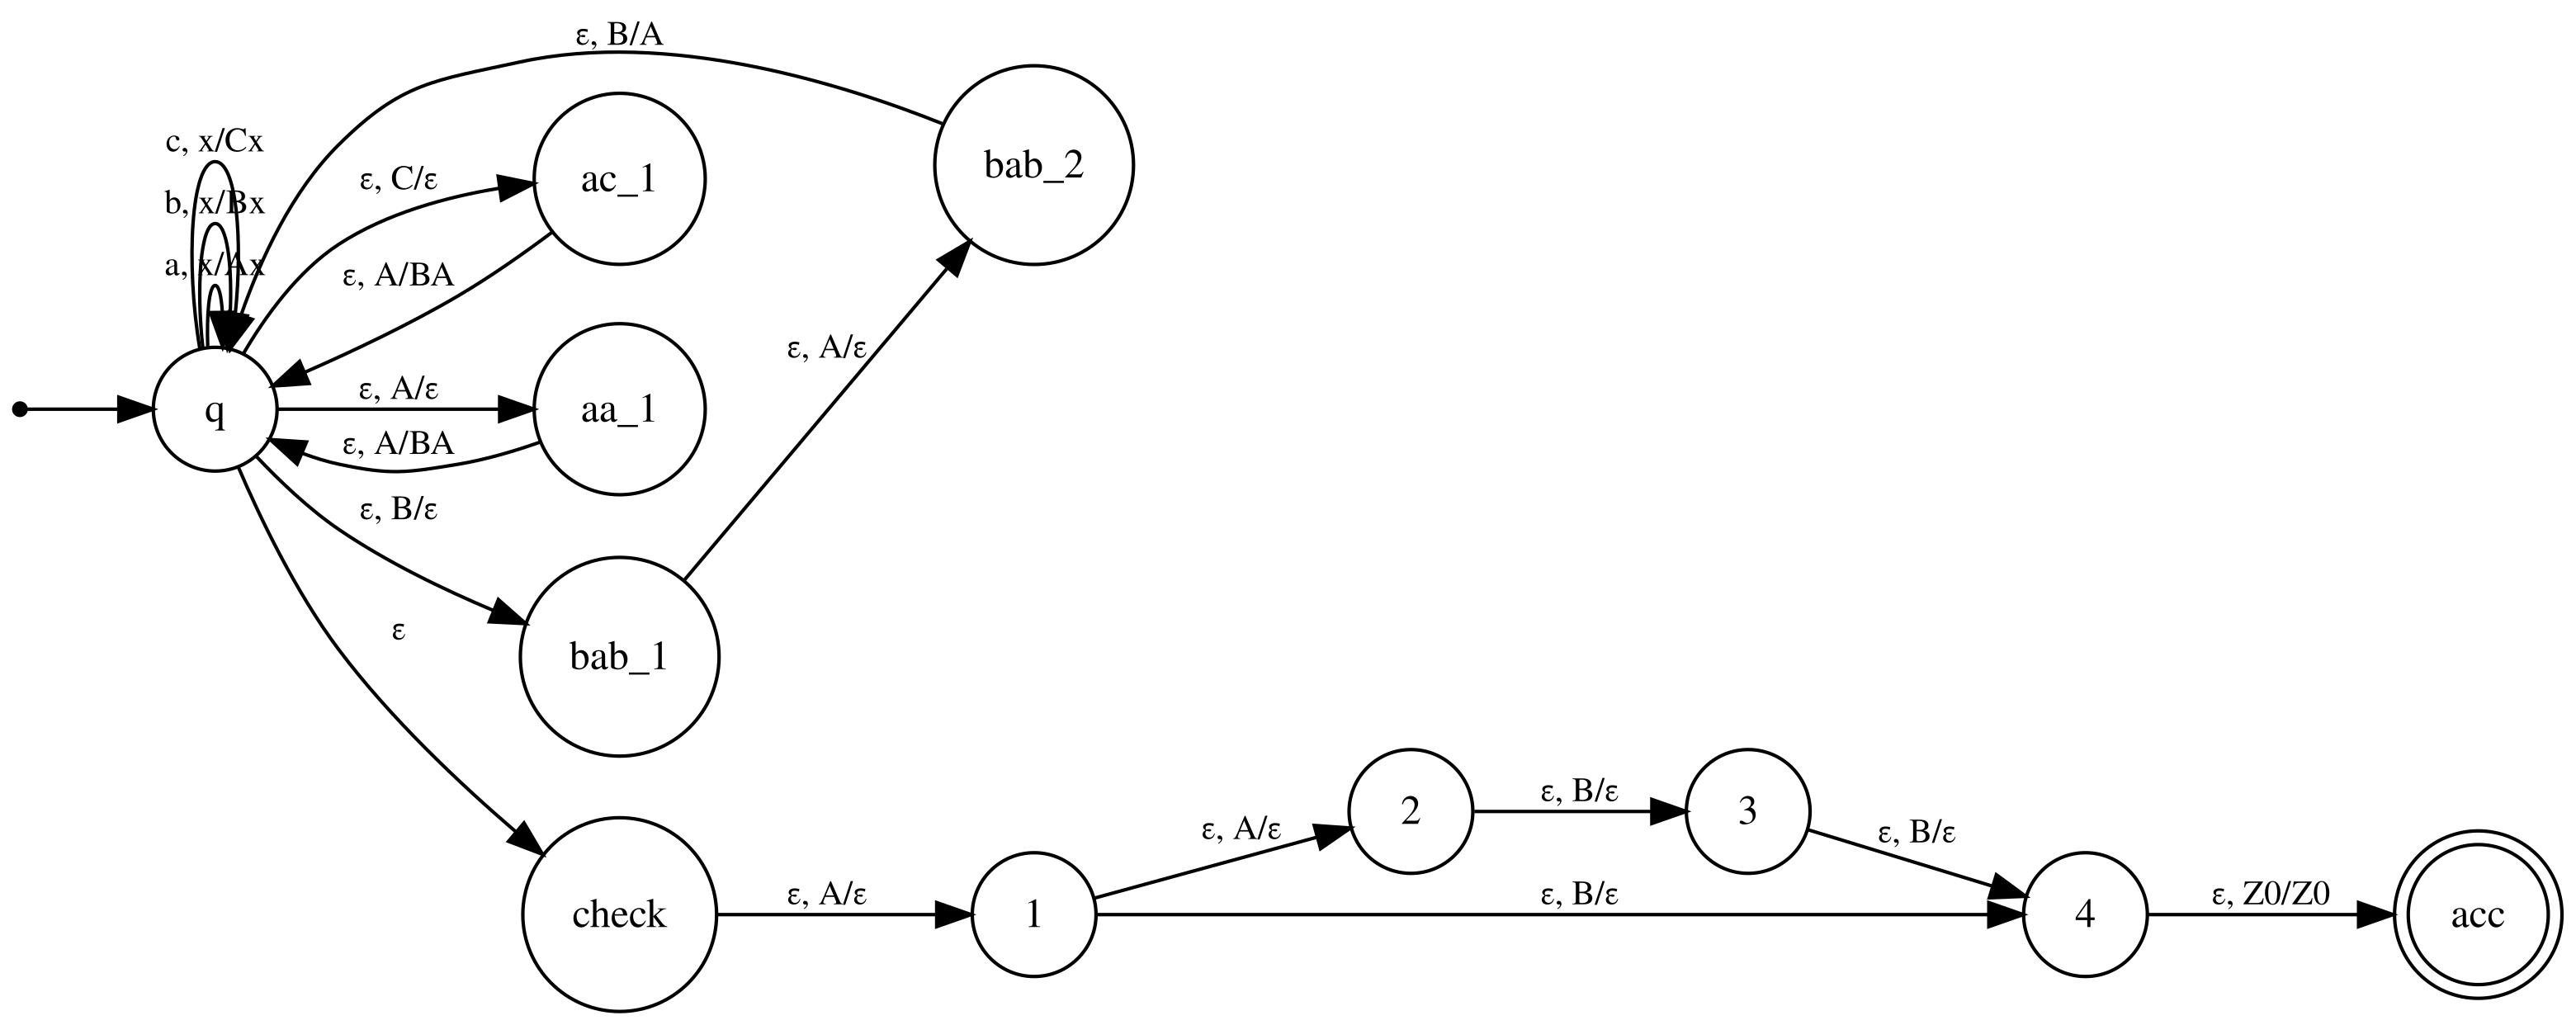
\includegraphics[width=\textwidth]{images/pda.png} 
\end{figure}

Рассмотрим $b^{2p}a^{2p}$. Пусть длина накачки - $p$. $|xy| \leq p \Rightarrow y$ содержится в $b^{2p}$. Тогда $xy^kz$ - это $b^{2p+i}a^{2p}$. Количество $b$ больше, чем количество $a \Rightarrow xy^kz$ не принадлежит языку $\Rightarrow$ язык нерегулярен.

\section{Задача 2}

$\{\omega \; \big{|} \; |\omega|_{ab} = |\omega|_{baa} \vee \omega = \omega^R \}$. Алфавит $\{a,b\}$.

Возьмем R = $ab(a|b)^*ba$. Пусть $\omega \in R \Rightarrow |\omega|_{ab} = |\omega|_{ba}$; $|\omega|_{baa} = |\omega|_{ba} - |\omega|_{bab} - 1 \leq |\omega|_{ba} - 1 = |\omega|_{ab} - 1$; $|\omega|_{baa} < |\omega|_{ab}$
$\Rightarrow \{\omega: |\omega|_{ab} = |\omega|_{baa} \} \cap R = \varnothing \Rightarrow L \cap R = \{\omega = \omega^R\} \cap R$

$L \cap R = \{abuba \; | \; u = u^R \}$.
Пусть L - DCFL. Тогда $L \cap R$ - тоже DCFL, но язык палиндромов не является детерминированным $\Rightarrow$ L - не DCFL.

\section{Задача 3}
\begin{figure}[h] 
\    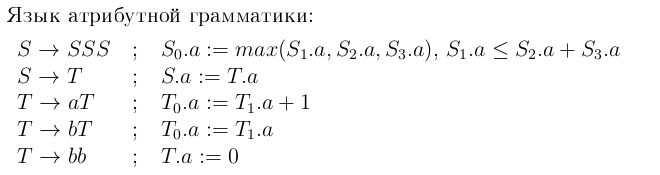
\includegraphics[width=0.8\textwidth]{images/t3.png} 
\end{figure}


$L(T) = (a|b)^*bb$, атрибут a считает число букв a в слове, $L(T) \subseteq L(S)$.
Предикат из $S \rightarrow SSS$ не исключает ни одного слова $\omega \in L(T)$. Кроме того, все выводы из S дают слова, оканчивающиеся на $bb$, то есть $L(S) \subseteq (a|b)^*bb$. Таким образом, $L(S) = (a|b)^*bb \Rightarrow$ язык КС и регулярный.

\end{document}

